\documentclass[a4papper]{article}

\usepackage[final]{pdfpages}
\usepackage{graphicx}
\usepackage{amssymb, amsmath, amsthm, mathrsfs}
\usepackage{indentfirst}
\usepackage{amsmath}
\usepackage{listings}
\usepackage{amsfonts}
\usepackage{wasysym}
\usepackage{stmaryrd}
\newtheoremstyle{neosn}{0.5\topsep}{0.5\topsep}{\rm}{}{\sc}{.}{ }{\thmname{#1}\thmnumber{ #2}\thmnote{ {\mdseries#3}}}
\theoremstyle{neosn}
\newtheorem{problem}{Problem}
\newtheorem{example}{Example}

\begin{document}
    \begin{center}
    {\bf Homework 6} \\
        \today \\
        TangLin
    \end{center}

    \problem{Prove that the problem of finding out whether an algebraic expression(with integer
        coefficients,addition and multiplication signs, and parentheses) is not identically
        zero (i.e. taking a nonzero value for some real values of the variables) belongs to NP.}\\
    \\
    Solution: \\
    \\
    It is obviously that we can build a DTM $M$ to certificate that the value of algebraic expression
    on a certain input vector of these variables.
    Without loss of generalities, we can only focus on the integer input vectors.
    If the algebraic expression with nonzero value, so there will be some integer vectors that make
    the value of the expression nonzero. \\

    Now we build machine $M$. \\

    First, we need to ensure input size, assume that our input is $exp\#\vec{x}$, and $len(exp \# \vec{x}) = n$.
    So $len(exp) \leqslant n$ and $len(\vec{x}) \leqslant n$.
    For conveniently calculating, we can transform the expression into a prefix expression.
    And it can be performed in polynomial time $p_1(n)$. \\
    Then we get the prefix expression, and we need to copy all the values which are in vector $\vec{x}$
    to the corresponding position in the prefix expression.
    If there are $m$ variables, then
    \[
        \sum_{i=1}^n len(x_i) = len(\vec{x})
    \]
    and for any $i$
    \[
        len(x_i) < len(\vec{x}).
    \]

    So we need
    \[
        \sum_{i=1}^n len(x_i)^2 < len(\vec{x})^2 \leqslant n^2
    \]
    steps to copy them. \\

    We got the prefix expression with values of all variables, then we will calculate it.
    We have $m$ variables, so there must be $m-1$ operators including $+$ and $\cdot$ in
    the expression.
    We know that all the $+$ and $\cdot$ operations can be performed in square time, so
    we need at most
    \[
        \begin{array}{l}
            len(x_1)^2 + (len(x_1)+len(x_2))^2 + \cdots + (len(x_1)+\cdots + len(x_m))^2 \leqslant \\
            \leqslant m \cdot (len(x_1)+\cdots + len(x_m))^2 \leqslant \\
            \leqslant len(\vec{x}) \cdot len(\vec{x})^2 \leqslant \\
            \leqslant n^3
        \end{array}

    \]

    So, totally, we need at most
    \[
        p_1(n) + n^2 + n^3
    \]
    and it is a polynomial.
    So this problem can be certificated in polynomial time and is in class \textbf{NP}. \\

    \\
    \\

    \problem{Prove that the following problem is \textbf{NP}-complete.\\
    Known condition: A finite family of finite sets (consisting of natural numbers) and
    a natural number $k$. \\
    Question: Is there a subfamily consisting of $k$ pairwise disjoint sets?
    } \\

    Solution: \\

    \\

    To prove it, we need to reduce some known \textbf{NP}-complete problem to this problem (PDS).
    So we need to find some similarities between the known problem and our problem.
    Here I find that Independent Set is very similar to the problem which we want to prove. \\

    First, we have to show that PDS $\in$ \textbf{NP}. \\
    Assume that there is a finite family of finite sets $In$
    \[
        In = \{S_1, S_2, S_3, \cdots, S_m\}
    \]
    where $S_i$ is a set consisting of natural numbers.
    And $Ce$ is a certification
    \[
        Ce = \{S_{i_1}, S_{i_2}, \cdots, S_{i_k}\}
    \]
    where $1 \leqslant i_j \leqslant m$ and $\forall r,s$ if $r \neq s$ then $i_r \neq i_s$.
    Assume that the length of binary string of $In$ is $len(In) = n$, then we have $m \leqslant n$,
    and $|S_i| \leqslant n$, where $|S_i|$ indicates the number of elements of set $S_i$. \\
    The first step to certificate $Ce \subset In$.
    We have known that we need square time to verify that two integers are equal.
    So we need at most
    \[
        n^2 \sum_{p=1}^k \sum_{q=1}^m |S_{i_p}| \cdot |S_q| \leqslant kmn^2 \leqslant n^4
    \]
    steps to check it. \\
    Then we need to answer whether all the elements in $Ce$ are mutually disjoint.
    We need at most
    \[
        n^2 \sum_{p,q=1;p \neq q}^k |S_{i_p}|\cdot |S_{i_q}| \leqslant k^2 \cdot n^2 \cdot n^2 \leqslant n^6
    \]
    So totally we need at most $n^4+n^6 \in O(n^6)$ steps to certificate it. \\
    So PDS $\in$ \textbf{NP}. \\

    Now we show that every Independent Set problem can be reduced to a PDS. \\

    Let undirected graph be $G=(V,E)$ and
    \[
        \begin{array}{l}
            V =  \{v_1, v_2, \cdots, v_m\} \\
            E =  \{(v_{i_1^1}, v_{i_1^2}), (v_{i_2^1}, v_{i_2^2}), \cdots , (v_{i_k^1}, v_{i_k^2})\}
        \end{array}
    \]
    where $v_{i_m^1}, v_{i_m^2} \in V$ for any $1 \leqslant m \leqslant k$. \\

    Let length of binary description of graph $G$ be $len(G) = n$.
    Obviously, $|V| < n$ and $|E| < n$.

    I will use idea of BFS to build the infinite family of infinite sets.
    For every vertex we can build a set consisting of natural numbers.

    We can start the construction on any vertex, here I will start with $v_1$.
    First, we construct a stack $H$ to store the vertexes which we are going to access and push
    $v_a$ into $H$.
    This operation needs at most $O(n)$ time (when the index of vertex are so large).
    Then we pop an element of $H$, and it needs at most $O(n)$ time.\\
    Then find all the neighborhoods of $v_1$ and push them into $H$, it needs $O(n)$ time,
    because we need search whole $E$.
    Then set $v_1$ a special status to indicate that it was visited.
    Assume that all the neighborhoods are
    \[
        \{v_{r_1}, v_{r_2}, \cdots, v_{r_p}\}
    \]
    where $p < n$.
    If there was some vertexes were visited, i.e. their special statuses were set, for example
    \[
        Visited = \{v_{r_{w_1}}, v_{r_{w_2}}, \cdots, v_{r_{w_t}}\}
    \]
    are visited, then build $S_a = \{a, r_{w_1}, r_{w_2}, \cdots, r_{w_t}\}$;
    if $Visited = \emptyset$, then $S_a = \{a\}$.
    It needs $O(n)$ time.
    Then repeat performance until $H$ is empty.\\
    Totally, we need $O(n^2)$ time.
    So we can build all the $m$ sets $S_i$ in $O(n^2)$ time.
    And the original problem which to find out the max independent set can be reduced to find
    the max mutually disjoint sets.
    Actually, we can also easily answer the question with given number $k$. \\
    So we can conclude that Independent Set $\leqslant_p$ PDS. So PDS is \textbf{NP}-complete. \\

    It is necessary to make an example of the whole building process.\\

    \example{Let $G=(V,E)$, where $E=\{v_1, v_2, v_3, v_4, v_5, v_6, v_7\}$ and
    $V=\{(v_1, v_2), (v_1, v_3), (v_1, v_4), (v_3, v_4), (v_3, v_5), (v_4, v_6), (v_4, v_7)\}$,
    then show the process of building set family.}


    \includepdfset{pagecommand={\thispagestyle{fancy}}}
    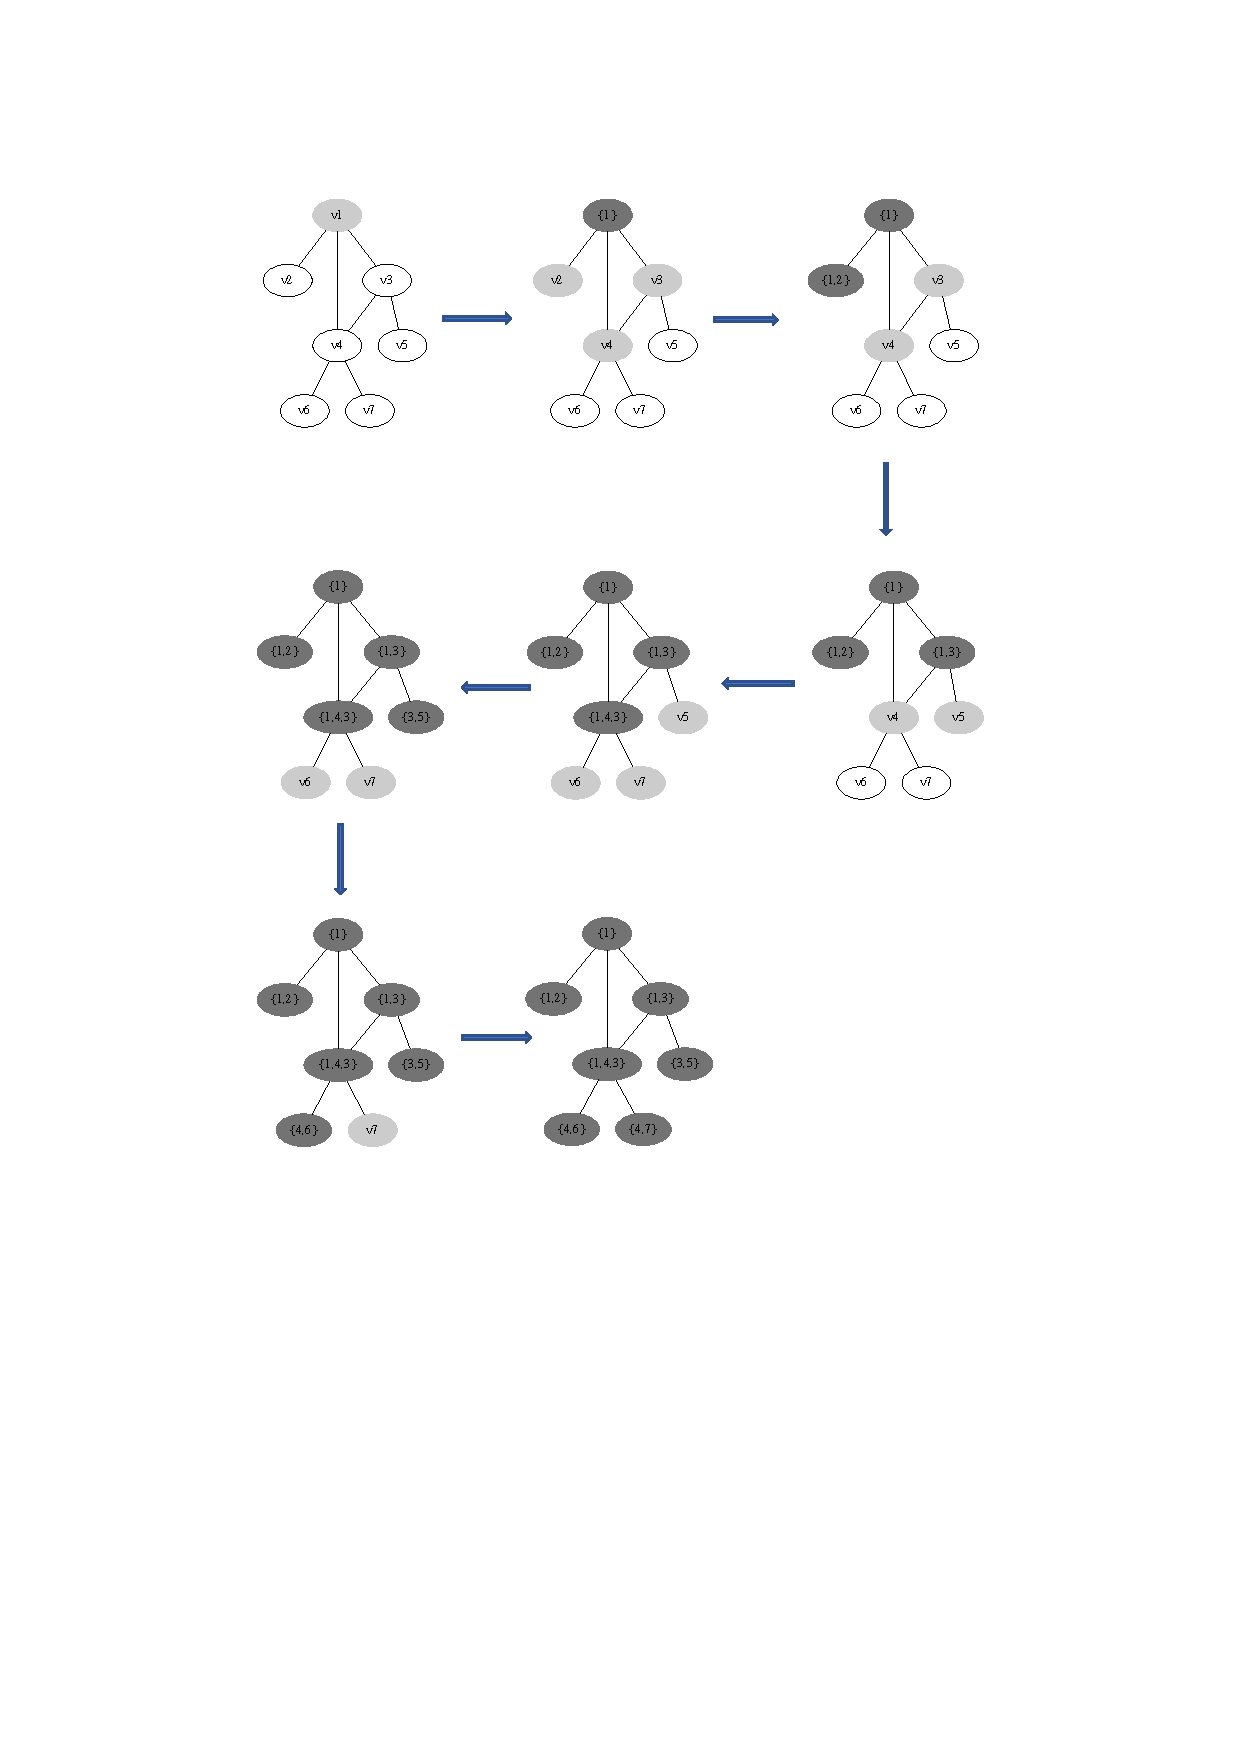
\includepdf{Example_Proc.pdf}


\end{document}